\documentclass{article}
\usepackage[portuges]{babel}
\usepackage[utf8]{inputenc}
\usepackage[T1]{fontenc}
\usepackage{graphicx}

\usepackage{float}
\usepackage{enumerate}
\usepackage{makeidx}
\usepackage{booktabs}
\usepackage{pdfpages}
\usepackage{a4wide}

\setlength\oddsidemargin{0.3in}
\setlength\evensidemargin{-0.3in}
\setlength\headsep{15pt}
\setlength\footskip{30pt}


% environment created for organization purposes, only.
\newenvironment{TODO}{%
  \color{blue} \itshape \begin{itemize}
}{%
  \end{itemize}
}

%---------------------------------------

% our addimage command
\newcommand{\addimg}[1]{%
  \begin{center}
    \includegraphics[width=0.75\textwidth]{#1}
  \end{center}
}

\newcommand{\RowStretch}[1]{\renewcommand{\arraystretch}{#1}}



%----------------------------------------------------------

\begin{document}

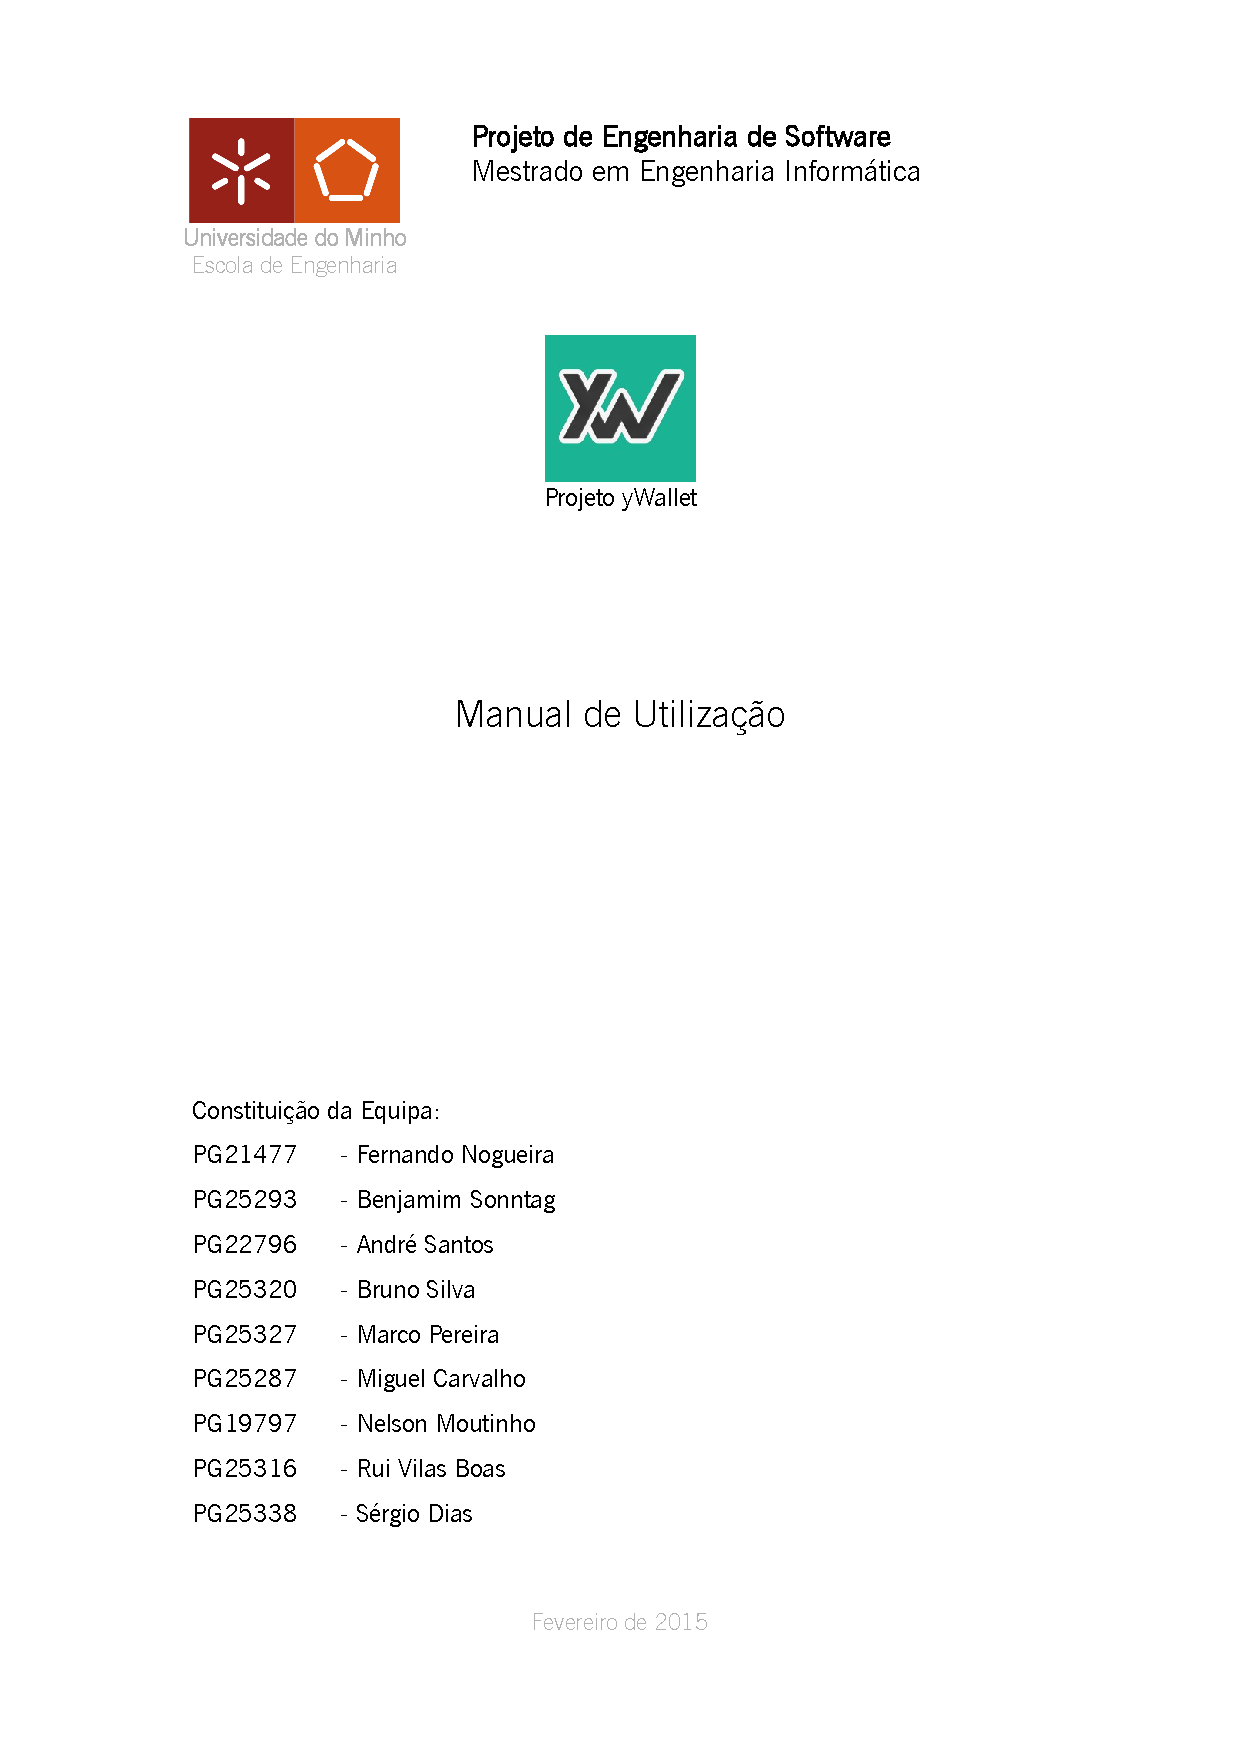
\includepdf[pages=-]{capa}

\tableofcontents

\pagebreak

\section{Autenticação}

  \begin{figure}[H]
    \begin{center}
      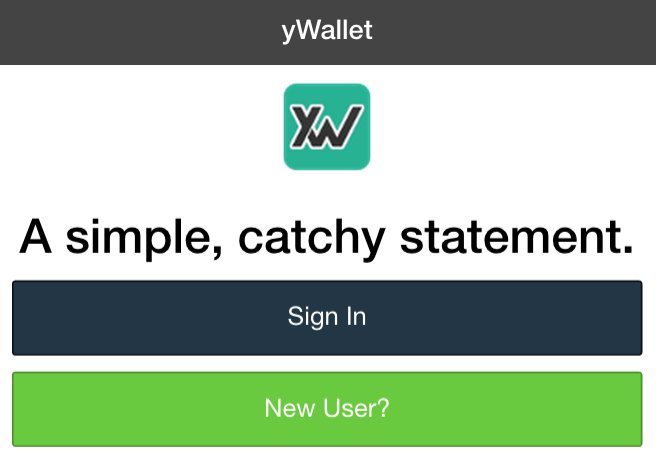
\includegraphics[width=0.75\textwidth]{authentication/init.png}
    \end{center}
    \caption{Arquitetura da plataforma}
    \label{fig:arq_app}
  \end{figure}

  \subsection{Registo}

  \subsection{Login}

  \subsection{Recuperar a \textit{Password}}

\section{\textit{Dashboard}}

\section{Conta}

\section{Mesadas}

\section{Pagamentos}

\section{Histórico}

\section{Notificações}

\section{Poupanças}

\section{Configurações}


\end{document}
